\section{Requirement and Overview}\label{sec:pilotstudy}


As surveyed in the Chapter~\ref{sec:relatedwork}, there are two main steps to augment node-link diagram: 1) extracting information from visualizations and their underlying data, 2) expressing the information to the end-users. Thus, we conducted pilot study aims to investigate the requirements for these two steps from the viewpoints of both three experts and twelve end-users. 
% Based on the literature review, we developed some sample graph description.
Based on the literature review, we collected some sample node-link diagrams.
Then we collected and summarized relevant feedbacks from 12 end-users and 3 visualization experts.


\subsection{Requirement Analysis}

We present our findings and concluded four requirements [E1-4] for information extraction and three requirements [D1-3] for information description. 

\noindent {\bf Extracting information.}

\begin{compactenum}[\textbf{E}1]
    \item {\bf Summarize Meanings of Data Entities.} Our experts suggested that the meanings of data entities (namely, nodes and links) should be explained to end-users. We found that
    end-users had less problems about the node meanings while they were confused on the meaning of links. End-user 1 mentioned ``what do links mean? Why are two nodes connected?''
    We suspected that it is due to the lack of link meanings in several collected cases.
    Thus, experts suggested us to focus on summarizing link meanings while ignore node meanings because they are usually explicitly defined in titles, captions, or legends.
    One of them explained that the meanings of links are finely defined as link conditions in various research~\cite{DBLP:journals/ivs/LiuNS14, DBLP:journals/ivs/HeerP14, DBLP:journals/tvcg/SrinivasanPEB18}. They represent how links are constructed according the nodes' attributes. Our approach should find the correct link condition among nodes automatically to help users understand the meaning of links.
    
    \item {\bf Extract visual encodings.} 
    Our end-users are attracted the visual encodings of nodes and links. 
    They are usually represented by legends in our collected cases.
    However, some of our participants were still confused on it. For example, some end-user mentioned that ``Legends are too concise to understand and even missed in some cases, which makes me confused about whether is there any information encoded.''
    Thus, Our approach should support constructing a totally mappings between visual channels and data attributes.
    
    \item {\bf Identify the layout type.} 
    % 节点链接图的布局几乎被我们一半以上的用户所忽略,因为他们缺少对图可视化的先验知识;然而,专家却认为布局是节点链接图必不可少的层面;
    Information about layouts in our cases were ignored by more than half of our users (7/12) due to their lack of prior knowledge. But some of them still paid attention to the layout. For example, the end-user 4 asked meanings of the length of a link, which actually asked the meanings of two nodes' distance.
    In contrast to the ignorance of end-users, our experts all agreed that the layout is essential to a node-link diagram and thus our approach should support extract the layout.
    Considering end-users' lack of prior knowledge, the experts believed that it is not suitable to explain the layout algorithm details to end-users. And the taxonomy~\cite{DBLP:journals/cgf/NobreMSL19} surveyed in Chapter~\ref{sec:relatedwork} are simple and meaningful for explaining the meanings of different layout: topology-driven layouts and attribute-driven layouts. Thus, they suggested us to identify whether the layout is topology-driven or attribute-driven or neither.
    
    \item {\bf Utilize multi-source inputs}. 
    % 页面呈现的内容有限,专家们建议,我们的方法需要能够利用多种方式的输入 ,特别是数据和可视化程序。这么做能够让我们收集的信息更加丰富和准确,从而避免误导用户。
    Information expressed by the user interface (e.g., web pages) is limited.
    Experts suggested our approach to utilize multi-source inputs, especially the origin data and the visualization program.
    Enriching the types of our inputs can improve the accuracy and the richness of the collected information to avoid misleading users.
\end{compactenum}

\noindent {\bf Describing information. }
\begin{compactenum}[\textbf{D}1]
    \item {\bf Describe the information via textual descriptions.} 
    Although some collected cases contain legends to interpret visual encodings, four of our end-users suggested more detailed hints such as textual descriptions to provide more comprehensive illustration. The end-user 4 said that ``Language is the bridge of communication, and language descriptions of visualizations can bridge me to their authors.'' 
    Thus, we choose textual descriptions to serve as a detailed hints, which is preferred by most of our non-professional participants and also chosen by various sophisticated visualization description generation research~\cite{DBLP:journals/tochi/FerresLST13, DBLP:conf/inlg/ObeidH20, DBLP:conf/apvis/LiuXHWY20}.
    
    \item {\bf Use templates to generate consistent descriptions.}
    One expert suggested that a template-based scheme is more suitable for our description generation, because it is stable and consistent to display simple information in our scenario. He also suggested us to highlight non-template information in the template to facilitate users' recognition.
    
    \item {\bf Organize descriptions according to their information.}
    One of our expert suggested us to organize descriptions according to their relationships. For example, he said all descriptions of visual encodings should be displayed together without inserting other descriptions such as the meanings of data entities.
    Thus, we should organize descriptions according to the structure of information.

    \item {\bf Construct mapping between graph and descriptions.} 
    % 看了一些带有legend的case之后,一些被试认为这种静态的hints难以追踪它们所表达的信息;他们建议可以通过高亮hints的描述对象来进行提示,以便更快理解这些hints;
    After investigating some cases with legends, some end-users mentioned that such static hints obstructed their information tracking. They suggested us to build a linkage between our hints and the visualization. So that hovering on our hints (we choose template-based descriptions) or the visualization should toggle highlighting of the other.
    It would make our hints more targeted and reduce mismatches with the end-users' mental map.
    % Several of participants suggested the hints should support interactions such as linking between hints and the visualization, which would make hints more targeted and reduce mismatches with the end-users' mental map. One of them said that ``Hovering on a certain node to toggle its description can help me a lot''. With the linking between descriptions and the diagram, end-users without prior knowledge will be more clear about the target of descriptions. A common way to express the linking between two elements is the highlighting interaction. Hovering on descriptions or the visualization should toggle highlighting of the other.
\end{compactenum}

\subsection{\ApproachName~Overview} \label{sec:overview}

\begin{figure*}[t]
    \centering
    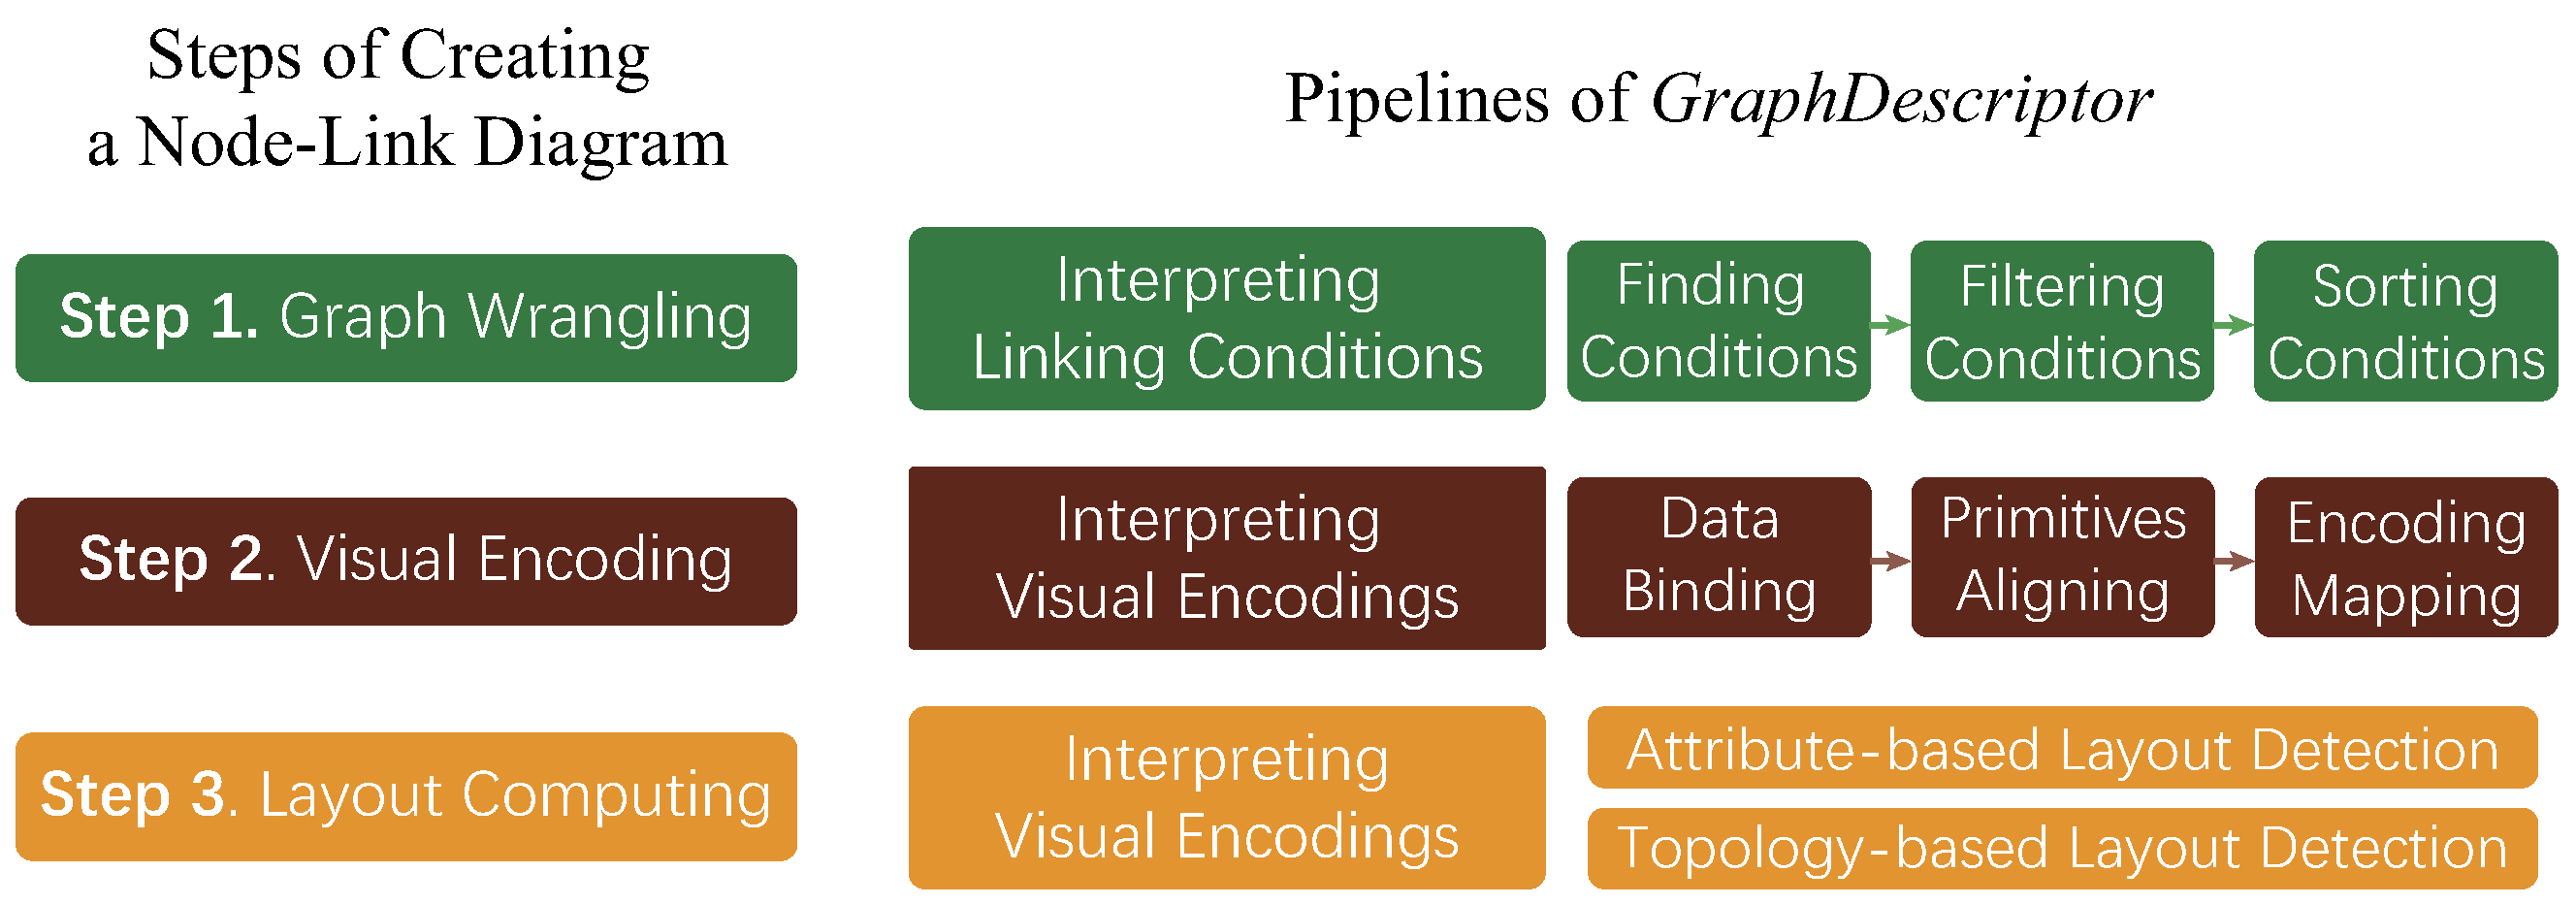
\includegraphics[width=2\columnwidth]{figures/workflow.eps}
    \caption{\ApproachName~consists of two parts: a) GraphExtractor and b) GraphDescriptor. GraphExtractor is used to extracting relevant information from node-link diagram, including meanings of links, visual encodings, and layout type. And GraphDescriptor is used to generating template-based descriptions with interactions. 
    }
    \label{fig:workflow}
\end{figure*}

Following the aforementioned requirements, we propose~\ApproachName~(Figure~\ref{fig:workflow}), an automatic description generation approach to augment the comprehensibility of node-link diagrams, which consists of three information extraction pipelines (GraphExtractor) and a linked description generator (GraphDescriptor). They work together to extract information from node-link diagrams and generate linked descriptions to express the information for end-users.

\noindent {\bf GraphExtractor: Information Extraction Pipelines} To complete \textbf{E1-4}, we design and implement three information extraction pipelines (Figure~\ref{fig:workflow}a) with multi-source inputs (\textbf{E}) including the captured visualization programs and the original graph data.

\begin{compactenum}[\textbf{P}1]
    \item {\bf Link Meanings Extraction Pipeline.}
    To implement \textbf{E1}, we summarize the link conditions. The pipeline takes the original graph data as input and selects proper conditions between connected node pairs to represent the link meanings.
    % to be specific, this pipeline consists of three main steps: 1) search candidate link conditions in every pairs of nodes; 2) filter out the wrong conditions; 3) store the remaining conditions with a priority, where a more detailed condition gets a higher ranking.
    
    \item {\bf Visual Encodings Extraction Pipeline.}
    Following \textbf{E2}, our pipeline forms the encoding scheme by extracting 1) mappings between data entities and visual elements and 2) correlations between data attributes and visual channels. It takes visualization programs and the original graph data as inputs and tests the relationship between the graph data and output visualizations to infer visual encodings.
    
    % It consists of three steps (Figure~\ref{fig:VisualEncodings}): 1) \textbf{data binding}: find the mapping between elements and data entities; 2) \textbf{elements aligning}: align elements according to their \textit{roles}; and 3) \textbf{encoding mapping}: detect correlations among attributes, elements, and visual channels.
    
    \item {\bf Layout Type Extraction Pipeline.} Based on \textbf{E3}, we propose this pipeline to determine whether the layout is attribute-based or topology-based. This function is handled in two steps: 1) capture the position of each node by computing bounding boxes and 2) determine the layout type by testing the Pearson correlation coefficient.
\end{compactenum}

\noindent {\bf GraphDescriptor: Description Generation Pipeline}. According to \textbf{D1-4}, we propose GraphDescriptor (Figure~\ref{fig:workflow}b) to express the information extracted by GraphExtractor to end-users. 
The description generation follows a manner of template-filling (\textbf{D1-2}). The sprite of the description is based on the extracted information, although the template bears a resemblance to the skeleton of the description.
To express the relationship of different levels of information (\textbf{D3}), We organize the generated descriptions in a pre-set structure. Besides, driven by \textbf{D4}, we link them to their corresponding visual elements to reach an interactive scheme. In this interactive scheme, when users hovering on the descriptions or visual elements, the other element will be highlighted.


% \textbf{Participants}. Our participants contains both experts and normal end users. Three experts (E1-3) are experts in graph visualization with five years experience. Twelve participants (P1-12) are all students or researchers who equip the basic knowledge of visualization but are with little experience of designing and implementing node-link diagrams. Their age varies from 22 to 32 ($SD = 3.00, M = 25.58$). Three of them are females. 

% \textbf{Procedure}. We showed the one of the three diagrams to each participant. We told the participants that the diagram is a node-link diagram. Their task was to describe the node-link diagram correctly. At the beginning, they have no knowledge about it. They can ask any question about the diagram and we give answers. The interview would continue until the participant said he fully understood it and described all its relevant information correctly. During the study, we collected their questions for further analysis.
% Finally, we asked them about their suggestions to improve the comprehensibility of node-link diagrams.



% \textbf{Dataset and proposed graph}. 
% \noindent 1) The \textbf{Movie-Actor-2019-China} graph (49 nodes and 99 links, Figure~\ref{fig:Movie-Actor-2019-China}a) was created to investigate the required information to explain the graph wrangling procedure and the layout. According to \textbf{A\ref{step:wrangling}}, we selected movies published in China from 2019 to 2020 as nodes and preserved seven attributes: ``title'', ``date-published'' (the publication date), ``actors'', ``genre'', ``director'', ``writer'', and ``country''. We connected all pairs of movies that shared the same actors and generated a ``common-actors'' attribute for each link to represent the number of the same actors between two movies. Then, according to \textbf{A\ref{step:layout}}, to investigate the information required to explain the layout, we pre-computed a layout with a spring layout algorithm~\cite{DBLP:journals/spe/FruchtermanR91} to reveal the relationships between two movies which include the same actor. Considering that visual encoding is not the point of this case, we only visualized nodes and links as the form of \texttt{<circle>}s and \texttt{<line>}s separately. Following \textbf{A\ref{step:encoding}} We used the color of the node encodes to present its publication season, and used the width of a link to encode its ``common-actors''. 

% \noindent 2) The \textbf{Movie-Actor-Jean-Pierre} graph (14 nodes and 25 links, Figure~\ref{fig:Movie-Actor-Jean-Pierre}a) was created to explore the information for explaining visual encodings and the layout. According to \textbf{A\ref{step:wrangling}}, we used the movies directed by Jean-Pierre Melville as an example. We selected these movies as nodes and connected two nodes when their corresponding movies have the same actors. To explore the information of interpreting visual encodings, we generated a node-link diagram with slightly more complex visual encodings. Considering the two kinds of layouts categorized by~\cite{DBLP:conf/biovis/PartlKLKSS12}, we employed an attribute-based layout following \textbf{A\ref{step:layout}}. The x and y coordinates encode the attribute ``year'' and ``duration'', respectively. Following \textbf{A\ref{step:encoding}}, we used circular and square nodes to encode movies published in France and Italy. For each node, the size encodes the number of votes (the attribute ``votes'') they have received; the color encodes their primary genres (the first genre in the list attribute ``genre''). 

% \noindent 3) The \textbf{Actor-Movie-2016-2021-China} graph (17 nodes and 55 links, Figure~\ref{fig:teaser}a) is designed to interpret how users understand a node-link diagram with complex visual design. Following \textbf{A\ref{step:wrangling}}, we first selected movies in the dataset that were only released in China from 2016 to 2021.
% We selected actors who have acted in more than five movies as nodes. We preserved five attributes for nodes: ``name'', ``movies'' (movies s/he acted in from 2016 to 2021), ``avg-vote'' (the average vote), ``votes'' (the number of votes s/he got), and ``number-of-movies-by-year'' (the number of movies the actor acted in each year from 2016 to 2021). We connected two actors who have acted in the same film together. 
% To complete \textbf{A\ref{step:layout}}, we used the x-coordinate to encode the attribute ``votes'', and the y-coordinate encodes the ``avg-vote''.
% To generate a complex visual design following \textbf{A\ref{step:encoding}}, we took inspiration of the node-link diagram created by Junker et al.~\cite{DBLP:journals/bmcbi/JunkerKS06}, and nested a simple bar chart into each node to show the number of movies the actor acted in from 2016 to 2021. 
% We used the width of a link encodes its attribute ``number-of-shared-movies''. We utilized the layout to show two attributes (``avg-vote'' and ``votes'') of each node. 

% , specifically, 1) \textbf{what} information should be extracted and 2) \textbf{how} to express it. Besides, to make our system both professional and easy to use by ordinary users, we would like to understand the requirement 

% from the viewpoints of both experts and end-users viewpoints. Thus, our study is two-fold, including expert workshop and end-user interview. Based on the findings from the workshop and interview, we formed the system requirement to guide the following pipeline design

% \subsection{Expert Workshop}

% We held a one-hour online expert workshop and invited three experts (E1-3) in graph visualization. Because the targeted users of our approach is normal user, we focus on the first step, namely feature extraction, to discuss. Experts provide three noteworthy aspects for extracting information:

% To understand the possible information we should extract to formulate descriptions, we need to clarify the procedure of creating a node-link diagram.

% , two of whom have focused on graph visualization research for more than five years. We recorded the the whole discussion through cameras and voice recording equipment for further organization and analysis. 

% The expert workshop provides three key steps of creating node-link diagram and suggests three noteworthy aspects for extracting information:

% \begin{compactenum}[\textbf{A}1]

% % \item {\bf Starting with graph wrangling.} Data preprocessing, namely graph data generating, should be carried out before feature extraction, however, this step often be overlooked. All experts highlight the need of deriving the relationship between nodes to form the information of link. E1 mentioned that ``Most of the time, we manipulate the graph data directly because it has been wrangled before. yet, not all the time the data has been preprocessed.'' 

% % He also gave an example of the well-known graph data from Les Miserables~\cite{knuth1993stanford}, which was generated by connecting characters that appear in one chapter. \label{step:wrangling}

% \item {\bf Encoding the basivisual elements}

% \item {\bf Extracting the meaning of layout}

% The \textbf{layout} is an essential step for creating node-link diagrams. During the workshop, all experts agreed that the layout is the key step of graph visualization and suitable layout could present the relationships of nodes and enhance the overall readability. They discussed several graph visualization tools, including Gephi~\cite{DBLP:conf/icwsm/BastianHJ09}, Cytoscape~\cite{DBLP:journals/bioinformatics/FranzLHDSB16}, and D3~\cite{DBLP:journals/tvcg/BostockOH11}.
% They said that these visualization tools solved two critical aspects of visualizing a graph: the layout and the visual encoding. Then experts give more detailed insights about layout. E2 mentioned that ``Layout algorithms calculate positions of nodes to show relationships between nodes on a two-dimensional plane. Almost all of them aim to reflect relationships between nodes in the graph data''.
% E1 added that ``There are also many algorithms with different goals, such as drawing layered and orthogonal diagrams, but they indeed aim to reflect the topology, namely, the readability''. E3 also mentioned that a survey~\cite{DBLP:journals/cgf/NobreMSL19} identifies a class of layouts as attribute-based layouts, which determine positions of nodes by attribute values. \label{step:layout}


% \item \textbf{Visual encodings} are not necessary but significant for visualizing the features of nodes and links. Besides visualizing the topology, visual encodings on nodes and links (e.g., encoding the category of nodes with their colors) extend the space of graph visualization. Thus patterns besides the topology can also be observed. E1 with experience in multivariate graph visualization mentioned that ``Occasionally, people draw nodes or links as glyphs to encode more attributes on node-link diagrams. A certain number of researchers are working on such kind of visualization for multivariate graphs''. \label{step:encoding}

% \end{compactenum}

% Besides, experts also discussed edge bundling techniques, interactions, attribute transformation, and several related topics. However, we only reported node-link diagram visualization related opinions in this paper.

% The three aspects are generic for most node-link diagrams. Thus, understanding what has happened belong these steps is essential to understand diagrams. Next, we design a new study to explore the detail information contained in the node-link diagrams created by these steps.


% \begin{figure}[t]
%     \centering
%     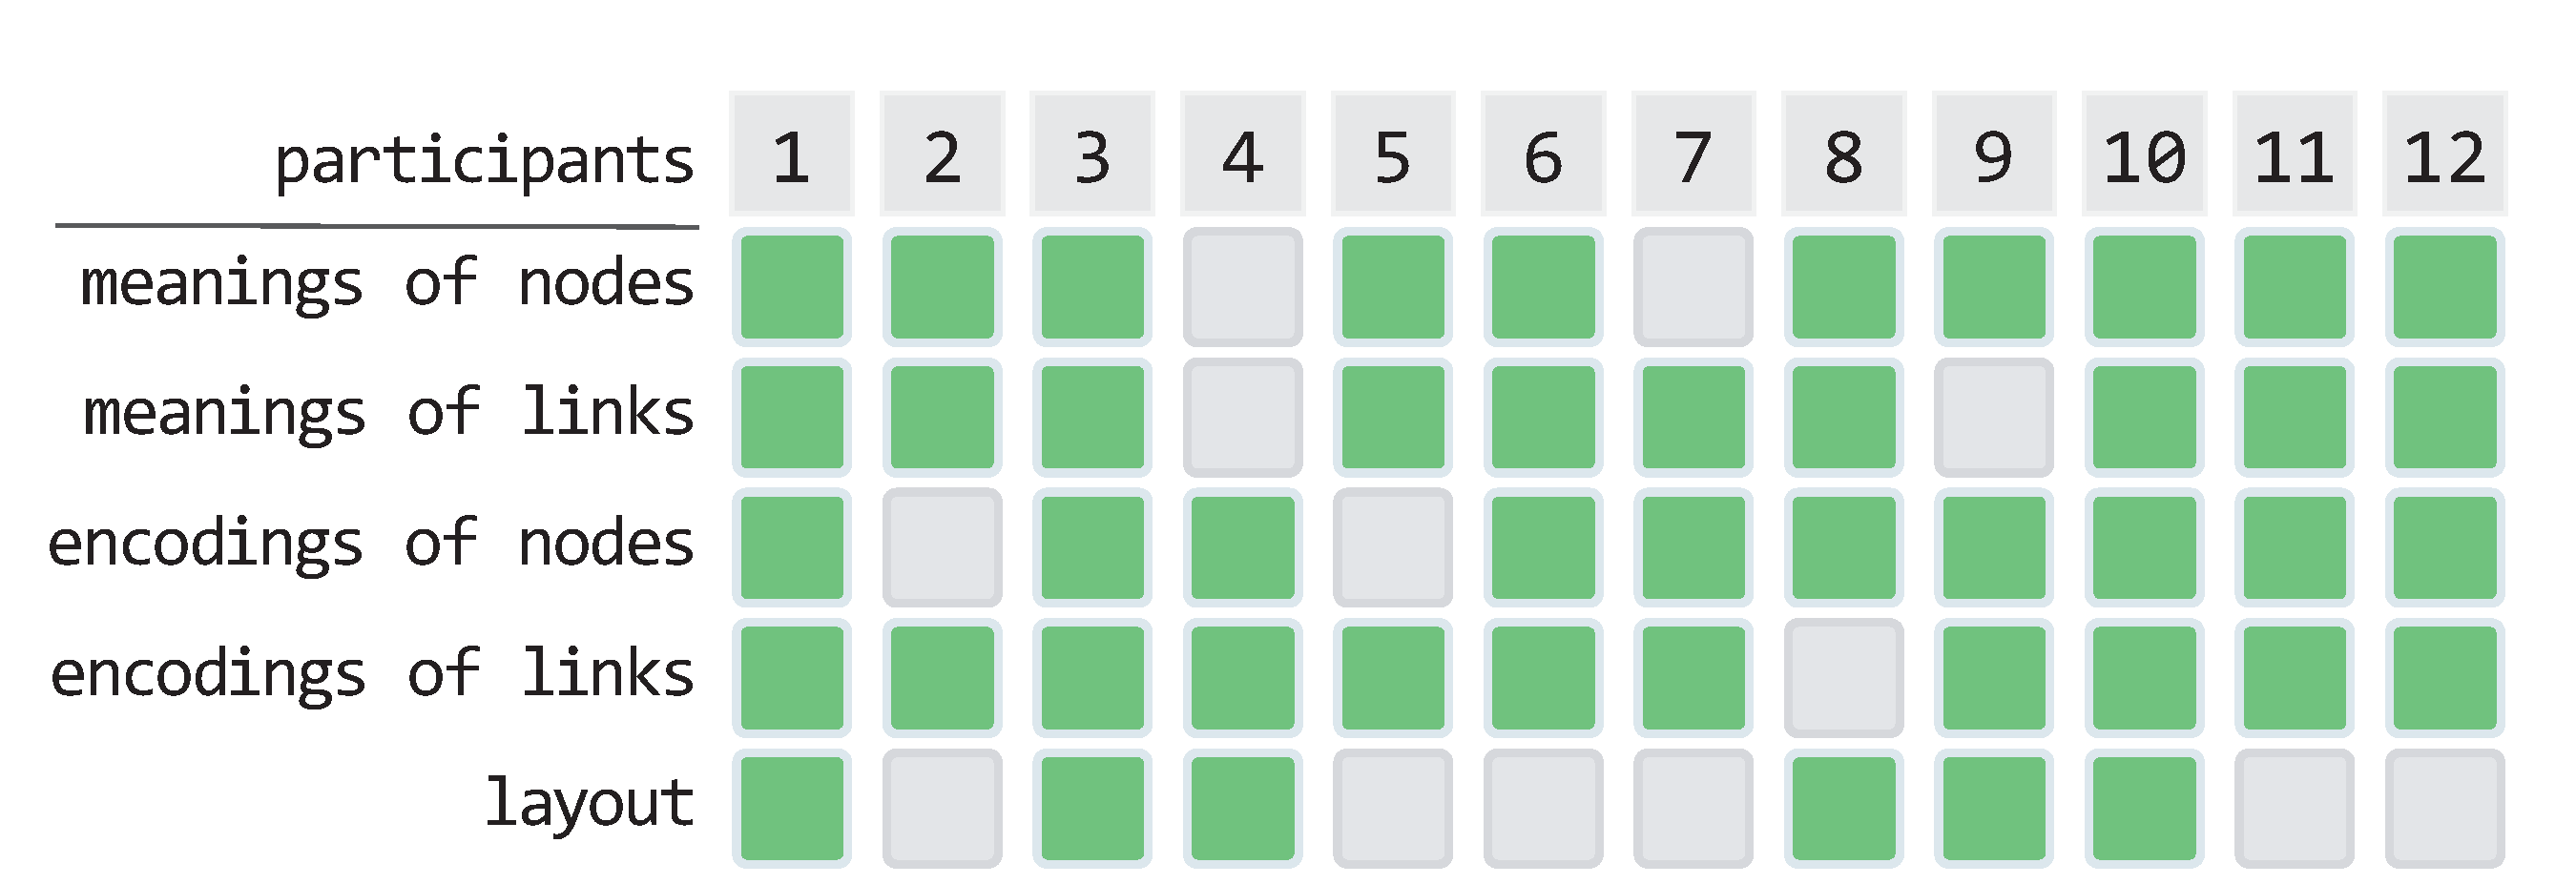
\includegraphics[width=1\columnwidth]{figures/UserInterview.eps}
%     \caption{A bitmap shows an overview of our user interview's results. Numbers (one to twelve) over the bitmap mean the numbers of participants. A green bar means the participant proposed confusions about the information.}
%     \label{fig:UserInterview}
% \end{figure}

% \subsection{User Interview}




% % 为了实现一个高可用的方法,我们不应该依赖用户来提供输入;但考虑到节点链接图的复杂性,没有任何输入或者仅仅有可视化结果是很难用来完成前三个需求的;所以,我们需要我们方法的输入是从用户角度出发易获得的,通过一些现有的工具就能够轻易获取;
% To implement a highly available approach for end-users, we should not require users to give inputs for our approach.
% Considering such characteristic, we form our requirement four as:
% \noindent \framebox{\parbox{\dimexpr\linewidth-2\fboxsep-2\fboxrule}{{\bf \labelR{easy-access}. The inputs of our approach should be easily accessible with current existing tools.} In today's web development environment, network traffic investigation tools can easily obtain the underlying data and web programs. Thus, our approach should only require such easily accessible inputs to reach a high availability.}}

% The first step of graph visualization is always the graph data generation. All experts reached an agreement that the graph wrangling is an important but easily overlooked part when creating node-link diagrams. E1 mentioned that ``Most of the time, the reason why we can directly manipulate the graph data is that it has been wrangled before, where links are derived from some relationships between nodes in the wrangling procedure.'' He also gave an example of the well-known graph data from Les Miserables~\cite{knuth1993stanford}, which was generated by connecting characters that appear in one chapter.

% \begin{itemize}
%     \item {\bf R1. graph wrangling should be extracted}
% \end{itemize}


% Visual encodings are not necessary but significant for visualizing the features of nodes and links. From the perspective of experts, visual encodings on nodes and links (e.g., encoding the category of nodes with their colors) extend the space of graph visualization. Thus patterns besides the topology can also be observed. E1 with experience in multivariate graph visualization mentioned that ``Occasionally, people draw nodes or links as glyphs to encode more attributes on node-link diagrams. A certain number of researchers are working on such kind of visualization for multivariate graphs''. From the perspective of end-users, they already confused by the enocodings of the nodes and links. For example, P1 said "what do red/square nodes mean/encode? What do the bar charts inside a node mean?" And P11 said "what does the thickness of the link mean? Is there any information encoded on links?" Based on their feedback, it is not difficult to find that visual encondings are improtant features that need to be extracted.

% \begin{itemize}
%     \item {\bf R2. visual encodings should be extracted}. Our approach should support constructing mappings between visual channels and data attributes.
% \end{itemize}

% The layout is an essential step for creating node-link diagrams. During the expert workshop, all experts agreed that the layout is the key step of graph visualization and suitable layout could present the relationships of nodes and enhance the overall readability. They discussed several graph visualization tools, including Gephi~\cite{DBLP:conf/icwsm/BastianHJ09}, Cytoscape~\cite{DBLP:journals/bioinformatics/FranzLHDSB16}, and D3~\cite{DBLP:journals/tvcg/BostockOH11}. They said that these visualization tools solved two critical aspects of visualizing a graph: the layout and the visual encoding. Then experts give more detailed insights about layout. E2 mentioned that ``Layout algorithms calculate positions of nodes to show relationships between nodes on a two-dimensional plane. Almost all of them aim to reflect relationships between nodes in the graph data''.
% E1 added that ``There are also many algorithms with different goals, such as drawing layered and orthogonal diagrams, but they indeed aim to reflect the topology, namely, the readability''. E3 also mentioned that a survey~\cite{DBLP:journals/cgf/NobreMSL19} identifies a class of layouts as attribute-based layouts, which determine positions of nodes by attribute values. The same thing also be observed and mentioned from the end-users. For the lack of experience, several participants misunderstood the conception of node-link diagrams. For example, the P4 asked meanings of the length of a link. And P7 mentioned "why are nodes placed in such a layout? What does the distance between two node mean?". In fact, the essence of his problem was the meaning of the layout. After we answered how nodes are placed, he finally understood the layout. Considering all these misunderstanding, we should extract the layout and explain them to the users.


% \begin{itemize}
%     \item {\bf R3. layout should be extracted}. Due to end-users' lack of prior knowledge, we found that it is more suitable to explain the meanings of different layout types to end-users rather than the layout algorithm details.
% \end{itemize}

% Surprisely, we found the meaning of nodes and links should be extracted from users' perspectives. Unlike experts, users cannot have a solid grasp of basic concepts. For example, P9 said "what do node mean/represent? what do data points represent?" and P11 said "what do links mean? Why are two nodes connected?"

% \begin{itemize}
%     \item {\bf R5. Meanings of nodes and links should be extracted}. Our approach should support extracting meanings of links automatically.
% Explaining meanings of nodes requires background knowledge about the dataset. We believe it is more suitable to explain nodes manually by visualization authors.  
% \end{itemize}


% \subsubsection{Information Expression}


% Most participants suggested different forms of hints such as text descriptions and legends to display the information they required to understand node-link diagrams.
% Most of them said simple descriptions can enhance their understanding such as ``The color of nodes encodes its ...''.
% P4 said that ``Language is the bridge of communication, language descriptions of a visualization can bridge me to visualization authors''.
% Thus we formulate our requirement as:
% % As non-professional users, most all our targeted users perfer  the system can express information by textual descriptions, which is also chosen by various sophisticated visualization description generation research~\cite{DBLP:conf/cvpr/KaflePCK18, DBLP:conf/apvis/LiuXHWY20, DBLP:conf/inlg/ObeidH20}.


% % \begin{itemize}
% %     \item {\bf R6. Expressing the extracted information by natural language}. Natural language is the most easy and natural way for end-users to understand.
% % \end{itemize}
% \noindent \framebox{\parbox{\dimexpr\linewidth-2\fboxsep-2\fboxrule}{{\bf \labelR{text-description}. Expressing the extracted information by textual descriptions}. We choose textual descriptions to convey information, which is preferred by most of our non-professional participants and also chosen by various sophisticated visualization description generation research~\cite{DBLP:conf/cvpr/KaflePCK18, DBLP:conf/apvis/LiuXHWY20, DBLP:conf/inlg/ObeidH20}.}}

% Several of participants suggested the hints should support interactions such as linking between hints and the visualization, which would make hints more targeted and reduce mismatches with the end-users' mental map. One of them said that ``Hovering on a certain node to toggle its description can help me a lot''. Thus, we formulate the requirement as:


% \noindent \framebox{\parbox{\dimexpr\linewidth-2\fboxsep-2\fboxrule}{{\bf \labelR{interactive-description}. Constructing linking between text descriptions and the node-link diagram}. 
% With the linking between descriptions and the diagram, end-users without prior knowledge will be more clear about the target of descriptions.
% A common way to express the linking between two elements is the highlighting interaction.
% Hovering on descriptions or the visualization should toggle highlighting of the other.}}

% \begin{itemize}
%     \item {\bf R6. Expressing the extracted information by interactive descriptions}. Our approach should support descriptions and interactions to express the extracted information. Descriptions are mature and sophisticated for explanation which are utilized by plenty of research~\cite{DBLP:conf/chi/KimHA20, DBLP:conf/inlg/ObeidH20, DBLP:journals/tochi/FerresLST13, DBLP:journals/coling/MittalMCR98}. And interactions are suggested by our participants to explain node-link diagrams. Thus, Our approach should support both descriptions and interactions.
% \end{itemize}



% 我想把结构重构,备份了一份在这儿,上面的估计改完就原版就看不出来了, 之前的结论太分散了,而且两边的意见没有整合过

% \subsection{Lessons learned and Design Recommendations}




% Finally, we summarized experts' viewpoints about the generation procedures into three key aspects:


% \noindent 1) The first step of graph visualization is always the \textbf{graph data generation}. All experts reached an agreement that the graph wrangling is an important but easily overlooked part when creating node-link diagrams. E1 mentioned that ``Most of the time, the reason why we can directly manipulate the graph data is that it has been wrangled before, where links are derived from some relationships between nodes in the wrangling procedure.'' He also gave an example of the well-known graph data from Les Miserables~\cite{knuth1993stanford}, which was generated by connecting characters that appear in one chapter.


% \noindent 2) The \textbf{layout} is an essential step for creating node-link diagrams. During the workshop, all experts agreed that the layout is the key step of graph visualization and suitable layout could present the relationships of nodes and enhance the overall readability. They discussed several graph visualization tools, including Gephi~\cite{DBLP:conf/icwsm/BastianHJ09}, Cytoscape~\cite{DBLP:journals/bioinformatics/FranzLHDSB16}, and D3~\cite{DBLP:journals/tvcg/BostockOH11}.
% They said that these visualization tools solved two critical aspects of visualizing a graph: the layout and the visual encoding. Then experts give more detailed insights about layout. E2 mentioned that ``Layout algorithms calculate positions of nodes to show relationships between nodes on a two-dimensional plane. Almost all of them aim to reflect relationships between nodes in the graph data''.
% E1 added that ``There are also many algorithms with different goals, such as drawing layered and orthogonal diagrams, but they indeed aim to reflect the topology, namely, the readability''. E3 also mentioned that a survey~\cite{DBLP:journals/cgf/NobreMSL19} identifies a class of layouts as attribute-based layouts, which determine positions of nodes by attribute values.


% \noindent 3) \textbf{Visual encodings} are not necessary but significant for visualizing the features of nodes and links. Besides visualizing the topology, visual encodings on nodes and links (e.g., encoding the category of nodes with their colors) extend the space of graph visualization. Thus patterns besides the topology can also be observed. E1 with experience in multivariate graph visualization mentioned that ``Occasionally, people draw nodes or links as glyphs to encode more attributes on node-link diagrams. A certain number of researchers are working on such kind of visualization for multivariate graphs''.


% Besides, experts also discussed edge bundling techniques, interactions, attribute transformation, and several related topics. However, we only reported node-link diagram visualization related opinions in this paper.


% The expert workshop provides three key steps of creating node-link diagram and suggests three noteworthy aspects for extracting information:
% 1) \textbf{graph wrangling}; 2) \textbf{layout computing}; 3) \textbf{visual encodings}. The three aspects are generic for most node-link diagrams. Thus, understanding what has happened belong these steps is essential to understand diagrams. Next, we design a new study to explore the detail information contained in the node-link diagrams created by these steps.

% \textbf{Result}. Participants' confusions suggested what information should be explained for them to understand.
% Solving their confusions provided us with a general idea to describe node-link diagrams.
% We identified the essential confusions and categorized them into five classes. Figure~\ref{fig:UserInterview} summarized the frequency of different types of confusions, and we listed question examples below:
% 1) \textbf{meanings of nodes}: e.g., what do node mean/represent? what do data points represent?
% 2) \textbf{meanings of links}: e.g.,  what do links mean? Why are two nodes connected?
% 3) \textbf{encodings of nodes}: e.g.,  what do red/square nodes mean/encode? What do the bar charts inside a node mean?
% 4) \textbf{encodings of links}: e.g.,  what does the thickness of the link mean? Is there any information encoded on links?
% 5) \textbf{layout}: e.g.,  why are nodes placed in such a layout? What does the distance between two node mean?
% For the lack of experience, several participants misunderstood the conception of node-link diagrams. For example, the fourth participant asked meanings of the length of a link. In fact, the essence of his problem was the meaning of the layout. After we answered how nodes are placed, he finally understood the layout.


% \textbf{Suggestions}.
% We also inquired about improvement suggestions from participants.
% Most participants suggested different forms of hints such as text descriptions and legends to display the information they required to understand node-link diagrams.
% Several of them suggested the hints should support interactions such as linking between hints and the visualization, which would make hints more targeted % 能够使得hints更具有针对性
% Considering our targeted end-users is non-professional users, we choose the express information by textual descriptions, which is also chosen by various sophisticated visualization description generation research~\cite{DBLP:conf/cvpr/KaflePCK18, DBLP:conf/apvis/LiuXHWY20, DBLP:conf/inlg/ObeidH20}.


% Following the questions raised by participants and their suggestions, we formulated the design requirements of our approach as: % expressing by extracting
% \begin{compactenum}[\textbf{R}1]
% \item \textbf{Extracting meanings of links}. Our approach should support extracting meanings of links automatically.
% Explaining meanings of nodes requires background knowledge about the dataset. We believe it is more suitable to explain nodes manually by visualization authors. \label{R:link}
% \item \textbf{Extracting visual encodings}. Our approach should support constructing mappings between visual channels and data attributes. \label{R:encoding}
% \item \textbf{Extracting layout types}. Due to end-users' lack of prior knowledge, we found that it is more suitable to explain the meanings of different layout types to end-users rather than the layout algorithm details. \label{R:layout}
% \item \textbf{Expressing the extracted information by interactive descriptions}. Our approach should support descriptions and interactions to express the extracted information. Descriptions are mature and sophisticated for explanation which are utilized by plenty of research~\cite{DBLP:conf/chi/KimHA20, DBLP:conf/inlg/ObeidH20, DBLP:journals/tochi/FerresLST13, DBLP:journals/coling/MittalMCR98}. And interactions are suggested by our participants to explain node-link diagrams. Thus, Our approach should support both descriptions and interactions. \label{R:description}
% \end{compactenum}




% generating understandable description based on extracted information, and 3) using a suitable interaction to express information to end-users ~\cite{DBLP:journals/ivs/CuiBYE19, DBLP:conf/diagrams/WuCEC10, DBLP:conf/icip/ZhouT00}. For the step two, considering our targeted end-users is non-professional users, we choose the express information by natural language, which is the most easy and natural way to understand. And there are already some sophisticated pipelines in NLP to generate descriptions by proving key words, which are already proved to have high usability and feasibility \cite{}. Thus, we choose to follow the existing and mature pipeline to convey information. Thus, our pilot study aims to investigate the step one and step three, specifically, 1) \textbf{what} information should be extracted and 2) \textbf{how} to express it. 

% To make our system both professional and easy to use by ordinary users, we would like to understand the requirement from the viewpoints of both experts and end-users viewpoints. Thus, our study is two-fold, including expert workshop and end-user interview.

% . First, we conducted an expert workshop, in which we clarified the creation procedure of a node-link diagram and relevant information contained. Second, we held a user interview to investigate how to explain node-link diagrams. 

% To be specific, we created three diagrams following the creation procedure. And then we showed these three diagrams to 12 participants, and we collected their feedback, especially confusions, to form the final design requirements.


